\documentclass[a4paper]{article}

%% Language and font encodings
\usepackage[english]{babel}
\usepackage[utf8x]{inputenc}
\usepackage[T1]{fontenc}

%% Sets page size and margins
\usepackage[a4paper,top=3cm,bottom=2cm,left=3cm,right=3cm,marginparwidth=1.75cm]{geometry}

%% Useful packages
\usepackage{amsmath}
\usepackage{graphicx}
\usepackage[colorinlistoftodos]{todonotes}
\usepackage[colorlinks=true, allcolors=blue]{hyperref}
\usepackage{wrapfig}

\hypersetup{
	urlcolor= blue,  %couleur des hyperliens
	linkcolor= black, %couleur des liens internes
}


\newcommand{\HRule}{\rule{\linewidth}{0.5mm}} % Defines a new command for the horizontal lines, change thickness here


\title{Cahier des charges}
\author{Andres Julien, Taylor Thomas}
\date{}
\begin{document}

\begin{titlepage}
\center


\includegraphics{incl/logo_sorbonne}\\[1cm] 

\HRule \\[0.4cm]
{ \huge \bfseries Robotique en essaim }\\
{ \huge \bfseries Cahier des charges}\\[0.4cm] % Title of your document
\HRule \\[1.5cm]



Julien \textsc{Andres}\\ % Your name
Thomas \textsc{Taylor}\\[3cm]

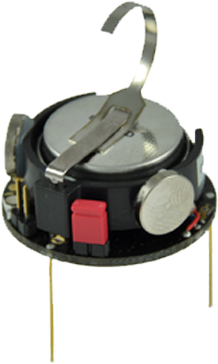
\includegraphics[width=4cm]{incl/Kilobots.png}



\end{titlepage}

\newpage
\renewcommand{\contentsname}{Sommaire}
\tableofcontents
\newpage
\section{Introduction}
\subsection{Contexte}

Ce document est le cahier des charges du projet \textit{Apprentissage en ligne et robotique en essaim (avec 100 robots Kilobots)}.
Réalisés au sein du master ANDROIDE de Sorbonne Université, les projets P-ANDROIDE consistent en la conception et la réalisation d'une application logicielle, se situant éventuellement dans le cadre d'une activité de développement plus importante. Les travaux sont faits en petites équipes (2 à 4 personnes, selon les projets proposés). Tout au long du travail, les étudiants sont encadrés par un enseignant-chercheur ou un chercheur associé à Sorbonne Université. Il s’agit d'acquérir une expérience pour le travail en équipe et la gestion de petits projets logiciels, ainsi que de se préparer à la rédaction de rapports et à la présentation orale d'un projet. \\

Nous sommes encadrés par Nicolas Bredèche, enseignant à Sorbonne Université et chercheur au sein du laboratoire Institut des Systèmes Intelligents et de Robotique (ISIR). L'ISIR est un laboratoire de recherche pluridisciplinaire qui rassemble des chercheurs et enseignants-chercheurs relevant de différentes disciplines des Sciences de l’Ingénieur et de l’Information ainsi que des Sciences du Vivant.

\subsection{Présentation du sujet}

La robotique en essaim est une branche de la robotique qui étudie la coordination de grandes populations de robots à comportements simples pour exécuter une tâche complexe. Elle s'inspire des colonies d'insectes sociaux, comme la fourmi ou l'abeille, qui peuvent réaliser des tâches en groupe, alors qu'un individu seul en est incapable. \\ Pour étudier la robotique en essaim, nous disposons d'une flotte de 100 Kilobots, un robot de 2 cm de diamètre pouvant communiquer via infrarouge et se déplacer à l'aide de deux moteurs à vibrations. Le but de ce projet est d'étudier plusieurs comportements fondamentaux tels que la couverture et l'agrégation et de les adapter aux Kilobots. Nous avons ensuite implémenté un algorithme d'apprentissage dit d'\textit{embodied evolution} dirigé par la pression environnementale, afin d'observer la dynamique adaptative de l'essaim en fonction de la structure de l'environnement.


\section{Description de la demande}
\subsection{Objectifs}

L'objectif de ce projet est d'implémenter des comportements collectifs pour un essaim de kilobots. Différents comportements doivent être fonctionnels (exploration, agrégation, couverture). Si le temps le permet, nous implémenterons un algorithme dit \textit{d'embodied evolution} dirigée par la pression environnementale, afin d'observer la dynamique adaptative de l'essaim en fonction de la structure de l'environnement. \\

Ce projet s'inscrit dans la continuité de l'utilisation des Kilobots à l'ISIR, l'un des principaux buts est la réutilisabilité et la facilité à prendre en main les outils que nous aurons réalisés pour aider les futurs utilisateurs. Ainsi, nous créerons un Docker qui contiendra les packages et applications à utiliser lors de la manipulation des Kilobots.

\subsection{Produit}

Les comportements réalisés lors du projet seront entièrement disponibles sur github à l'adresse
\url{https://github.com/JulienAndres/p_androidKilobot} et dans un Docker regroupant tout le code source et les applications permettant de le faire tourner.

\subsection{Comportements}

\subsubsection{Agrégation}

Les robots sont disposés aléatoirement dans l’arène et ne sont pas nécessairement tous
connectés. Lors du lancement du comportement, ils s’agrègent tous ensemble. Le but d'un robot est de s'approcher d'un voisin intéressant, i.e. celui qui a le plus de voisins, pour former un cluster.
En introduisant une probabilité de quitter le cluster auquel il appartient, il sera possible d'observer la formation de clusters plus ou moins grands selon les paramètres initiaux.

\subsubsection{Couverture}

Les robots sont rassemblés en un unique cluster. Lors du lancement du comportement, Les
robots s’éloignent alors les uns des autres afin d’occuper le plus grand espace possible dans l’arène
tout en restant à portée du groupe de robots.
Lorsque les robots sont suffisamment éloignés tout en restant connecté avec un Kilobot, le comportement arrive à stabilité.

\subsubsection{Embodied evolution}

Le but de l'embodied evolution est d'introduire au sein de la population de robots un algorithme évolutionnaire leur permettant de s'adapter à l'environnement. Chaque Kilobot possède donc un génome (jeu de paramètres) qu'il communique à ses voisins. A long terme, un génome peut être considéré performant si tous les robots restants l'ont adopté.

\section{Déroulement}

\subsection{Plan de route}

\begin{center}
    \begin{tabular}{ | p{5cm} | c | }
    \hline
    Tâche réalisée & Date\\ \hline
    Prise en main des Kilobots, familiarisation au code et étude du projet précédent  & 1/02/18\\ \hline
    Agrégation et couverture & 22/02/18\\ \hline
	Docker et documentation & 15/03/18\\ \hline
    Utilisation du bloc actif et des bandes de LED & 18/04/18\\ \hline
    Embodied evolution (mEDEA) & 3/05/18\\ \hline
    \end{tabular}
\end{center}

Ce tableau présente le plan de route destiné au développement des comportements des Kilobots, à la documentation ainsi qu'à la mise en place du Docker. Plusieurs tâches sont susceptibles d'être réalisées à la fois, certaines allant en paires et pouvant prendre plus ou moins de temps qu'anticipé.


\subsection{Ressources disponibles}

L'ensemble du code source est écrit en langage C, en utilisant la chaîne de compilation AVR. Avant validation, par souci de facilité, le simulateur Kilombo sera utilisé. Il sera donc important lors du développement de produire un code à la fois compatible avec kilolib et kilombo.
\\ \\
Nous disposons de blocs actifs que nous pouvons disposer dans l'environnement, chaque bloc émettant un signal infrarouge dans son voisinage, qui peut être utilisé pour communiquer avec les robots proches. Ce dispositif est aussi disponible sous forme de bandes de LED.

L'objectif principal étant d'observer les comportements sur robots réels, l'ISIR a mis à disposition un essaim de 100 Kilobots et le matériel nécéssaire à leur fonctionnement, ainsi qu'une arène de 2x2 mètres. 

\end{document}